\documentclass[mathserif,18pt,xcolor=table]{beamer}

% Load Beamer Style Theme
% TAMU Based
\usepackage{tamu_beamer}
\usepackage[font=small,skip=0pt]{caption}
\usepackage{etoolbox}
% \preto\subequations{\ifhmode\unskip\fi}
% \AtBeginEnvironment{subequations}{\ifhmode\unskip\fi}
% \AtBeginEnvironment{equation}{\ifhmode\unskip\fi}
\makeatletter
\g@addto@macro\normalsize{%
\setlength\abovedisplayskip{0pt}
\setlength\belowdisplayskip{0pt}
\setlength\abovedisplayshortskip{0pt}
\setlength\belowdisplayshortskip{0pt}
}
\makeatother


% Specifiy the location of images to be used
\graphicspath{{figures/}}


% Document Title Page
\title{Sommerfeld Integral}
\subtitle{Horizontally Oriented Magnetic Dipole above Silver Half-plane}
\author[Hasan Tahir Abbas]{ \underline{Hasan~Tahir~Abbas}}
\institute{Department of Electrical  \& Computer Engineering\\ \mbox{} \\ \pgfuseimage{tamuecenbig}}
\date[Spring 2017]{}
% \date[Spring 2017]{\today}

\begin{document}
\preto\subequations{\ifhmode\unskip\fi}
\AtBeginEnvironment{subequations}{\ifhmode\unskip\fi}
\AtBeginEnvironment{equation}{\ifhmode\unskip\fi}
% Draw Boxes in the footer with pertinent info
\tikzstyle{block} = [rectangle, draw, rounded corners, shade, top color=white, text width=5em,
bottom color=blue!50!black!20, draw=blue!40!black!60, very thick, text centered, minimum height=4em]
\tikzstyle{line} = [draw, -latex']
\tikzstyle{cloud} = [draw, ellipse,top color=white, bottom color=red!20, node distance=2cm, minimum height=2em]

% Tick Style
\beamertemplateballitem
% \beamertemplatetransparentcoveredhigh

\frame{\titlepage}


% Add TAMU logo on each slide in the north-east side
% Shifted to be right at the edge
\addtobeamertemplate{frametitle}{}{%
\begin{tikzpicture}[remember picture,overlay]
  \node[anchor=north east,yshift=5pt,xshift=2pt] at (current page.north east) {
\includegraphics[height=.7cm]{ecen}};
\end{tikzpicture}}




% ------------------------------------------------------------
% ------------------------------------------------------------
% ------------------------------------------------------------
% ------------------------------------------------------------
% ------------------------------------------------------------
% ------------------------------------------------------------
% ------------------------------------------------------------
\begin{frame}
  \frametitle{Theory}
  \framesubtitle{Thin Sheet Simulation}
  \begin{columns}[T] % align columns
    \begin{column}{.5\textwidth}
      \begin{itemize}
        \item{Volume Integral formulation}
      \end{itemize}
      \begin{equation} \nonumber
        \begin{split}
          \v A &= \frac{\u}{4 \pi} \int\limits_{V} \v J_v(\v r')  \frac{ e^{-j k_1 |\v r - \v r'|}}{|\v r - \v r'|} \diff{v'} \\
          \v E_1^{scat} &= -\frac{j \O}{k_1^2} \left( k_1^2 + \del \del \cdot \right) \v A \\
          \v J_v &= \frac{-j k_1}{Z_0}(\E_2 - 1)\v E_2
        \end{split}
        \label{eq:E1sc}
      \end{equation}
      \begin{itemize}
        \item{Surface current $J_s$ approximated from $J_v$}
      \end{itemize}
    \end{column}
    \begin{column}[T]{.5\textwidth}
      \vspace*{-2cm}
      \begin{itemize}
        \item{Impedance (Leontovich) Boundary Conditions}
      \end{itemize}
      \begin{equation} \nonumber
        \v E_{tan} = \eta Z_0 \hat{\v n} \times \v H
        \label{eq:eps}
      \end{equation}
      \begin{equation} \nonumber
        \begin{split}
          E^i &= \eta Z_0 J_s(x') \\
          & + \frac{\O \u}{4}  \int\limits_{l} J_s(x')  H_0^{(2)}(k_2 |x - x'|) \diff{x'}
        \end{split}
        \label{eq:eps}
      \end{equation}
      % Use this to preserve fonts from Inkspace
      \begin{figure}
        \def\svgwidth{.75\linewidth}
        \input{figures/seniors.pdf_tex}
        \caption{Dielectric Slab geometry}
      \end{figure}
      \end{column}%
    \end{columns}
  \end{frame}
  % ------------------------------------------------------------
  % ------------------------------------------------------------
  % ------------------------------------------------------------
  % ------------------------------------------------------------
  % ------------------------------------------------------------
  % ------------------------------------------------------------
  % ------------------------------------------------------------
  \begin{frame}
    \frametitle{Proposed Scheme}
    \framesubtitle{Surface Integral Equation}

    \begin{itemize}
      \item{Surface Equivalence Theorem}
    \end{itemize}
    \begin{figure}
      \centering
      \def\svgwidth{1\linewidth}
      \input{figures/equivalence.pdf_tex}
      \caption{(a). Actual and its equivalent models for the (b) external and, (c) Internal region }
    \end{figure}
  \end{frame}
  % ------------------------------------------------------------
  % ------------------------------------------------------------
  % ------------------------------------------------------------
  % ------------------------------------------------------------
  % ------------------------------------------------------------
  % ------------------------------------------------------------
  % ------------------------------------------------------------
  \begin{frame}
    \frametitle{Proposed Scheme}
    \framesubtitle{Surface Integral Equation}
    \vspace*{-.4cm}
    \begin{itemize}
      \item{Exterior Region}
    \end{itemize}
    \begin{equation} \nonumber
      \begin{split}
        \v E_1 &= \v E_i + \v E_1^{scat} \\
        &=  -\frac{\O}{4 k_1^2} \left( k_1^2 + \del \del \cdot \right) \int\limits_{C} \v J_s(\v p') H_0^{(2)}(k_1 |\v \p - \v \p'|) \diff{l'} \\
        &- \frac{1}{4 \E j} \del \x \int\limits_{l} \v M_s(\v \p') H_0^{(2)}(k_1 |\v \p - \v \p'|) \diff{l'} + \v E_i
      \end{split}
      \label{eq:E1sc}
    \end{equation}
    \begin{equation} \nonumber
      \begin{split}
        \v H_1 &= \v H_i + \v H_1^{scat} \\
        &= \frac{1}{4 j} \del \x \int\limits_{l} \v J_s(\v \p') H_0^{(2)}(k_1 |\v \p - \v \p'|) \diff{l'} \\
        &-\frac{\O}{4 k_1^2} \left( k_1^2 + \del \del \cdot \right) \int\limits_{l} \v M_s(\v \p') H_0^{(2)}(k_1 |\v \p - \v \p'|) \diff{l'} + \v H_i
      \end{split}
      \label{eq:H1sc}
    \end{equation}
  \end{frame}
  % ------------------------------------------------------------
  % ------------------------------------------------------------
  % ------------------------------------------------------------
  % ------------------------------------------------------------
  % ------------------------------------------------------------
  % ------------------------------------------------------------
  % ------------------------------------------------------------
  \begin{frame}
    \frametitle{Proposed Scheme}
    \framesubtitle{Surface Integral Equation}
    \vspace*{-.4cm}
    \begin{itemize}
      \item{Interior Region}
    \end{itemize}
    \begin{equation} \nonumber
      \begin{split}
        \v E_1 &= \v E_i + \v E_1^{scat} \\
        &=  -\frac{\O}{4 k_1^2} \left( k_1^2 + \del \del \cdot \right) \int\limits_{C} \left(-\v J_s(\v p')\right) H_0^{(2)}(k_1 |\v \p - \v \p'|) \diff{l'} \\
        &- \frac{1}{4 j} \del \x \int\limits_{l} \left(-\v M_s(\v \p')\right) H_0^{(2)}(k_1 |\v \p - \v \p'|) \diff{l'}
      \end{split}
      \label{eq:E1sc}
    \end{equation}
    \begin{equation} \nonumber
      \begin{split}
        \v H_1 &= \v H_i + \v H_1^{scat} \\
        &= \frac{1}{4 j} \del \x \int\limits_{l} \left(-\v J_s(\v \p')\right) H_0^{(2)}(k_1 |\v \p - \v \p'|) \diff{l'} \\
        &-\frac{\O}{4 k_1^2} \left( k_1^2 + \del \del \cdot \right) \int\limits_{l} \left(-\v M_s(\v \p')\right) H_0^{(2)}(k_1 |\v \p - \v \p'|) \diff{l'}
      \end{split}
      \label{eq:H1sc}
    \end{equation}
  \end{frame}
  % ------------------------------------------------------------
  % ------------------------------------------------------------
  % ------------------------------------------------------------
  % ------------------------------------------------------------
  % ------------------------------------------------------------
  % ------------------------------------------------------------
  % ------------------------------------------------------------
  \begin{frame}
    \frametitle{Field Computation}
    \framesubtitle{Layered media}
    \begin{columns} % align columns
      \begin{column}[T]{.5\textwidth}
        \begin{itemize}
          \item Difficulty in simulation of thin objects
          \item Dense mesh
          \item Computationally expensive
          \item No guarantee of correct solution
        \end{itemize}
        \begin{subequations}
          \begin{align}
            \v{\ti E}(\v{r}) = <{\ti {\tns G}}^{EJ} ; \v{\ti J}(\v{r'})>
            \label{eq:E_GJ}\\
            \v{\ti H}(\v{r}) = <{\ti {\tns G}}^{HJ} ; \v{\ti J}(\v{r'})>
          \end{align}
          \label{eq:EH_GJ}
        \end{subequations}
      \end{column}
      \begin{column}[T]{.5\textwidth}
        \begin{figure}[!t]
           \noindent
           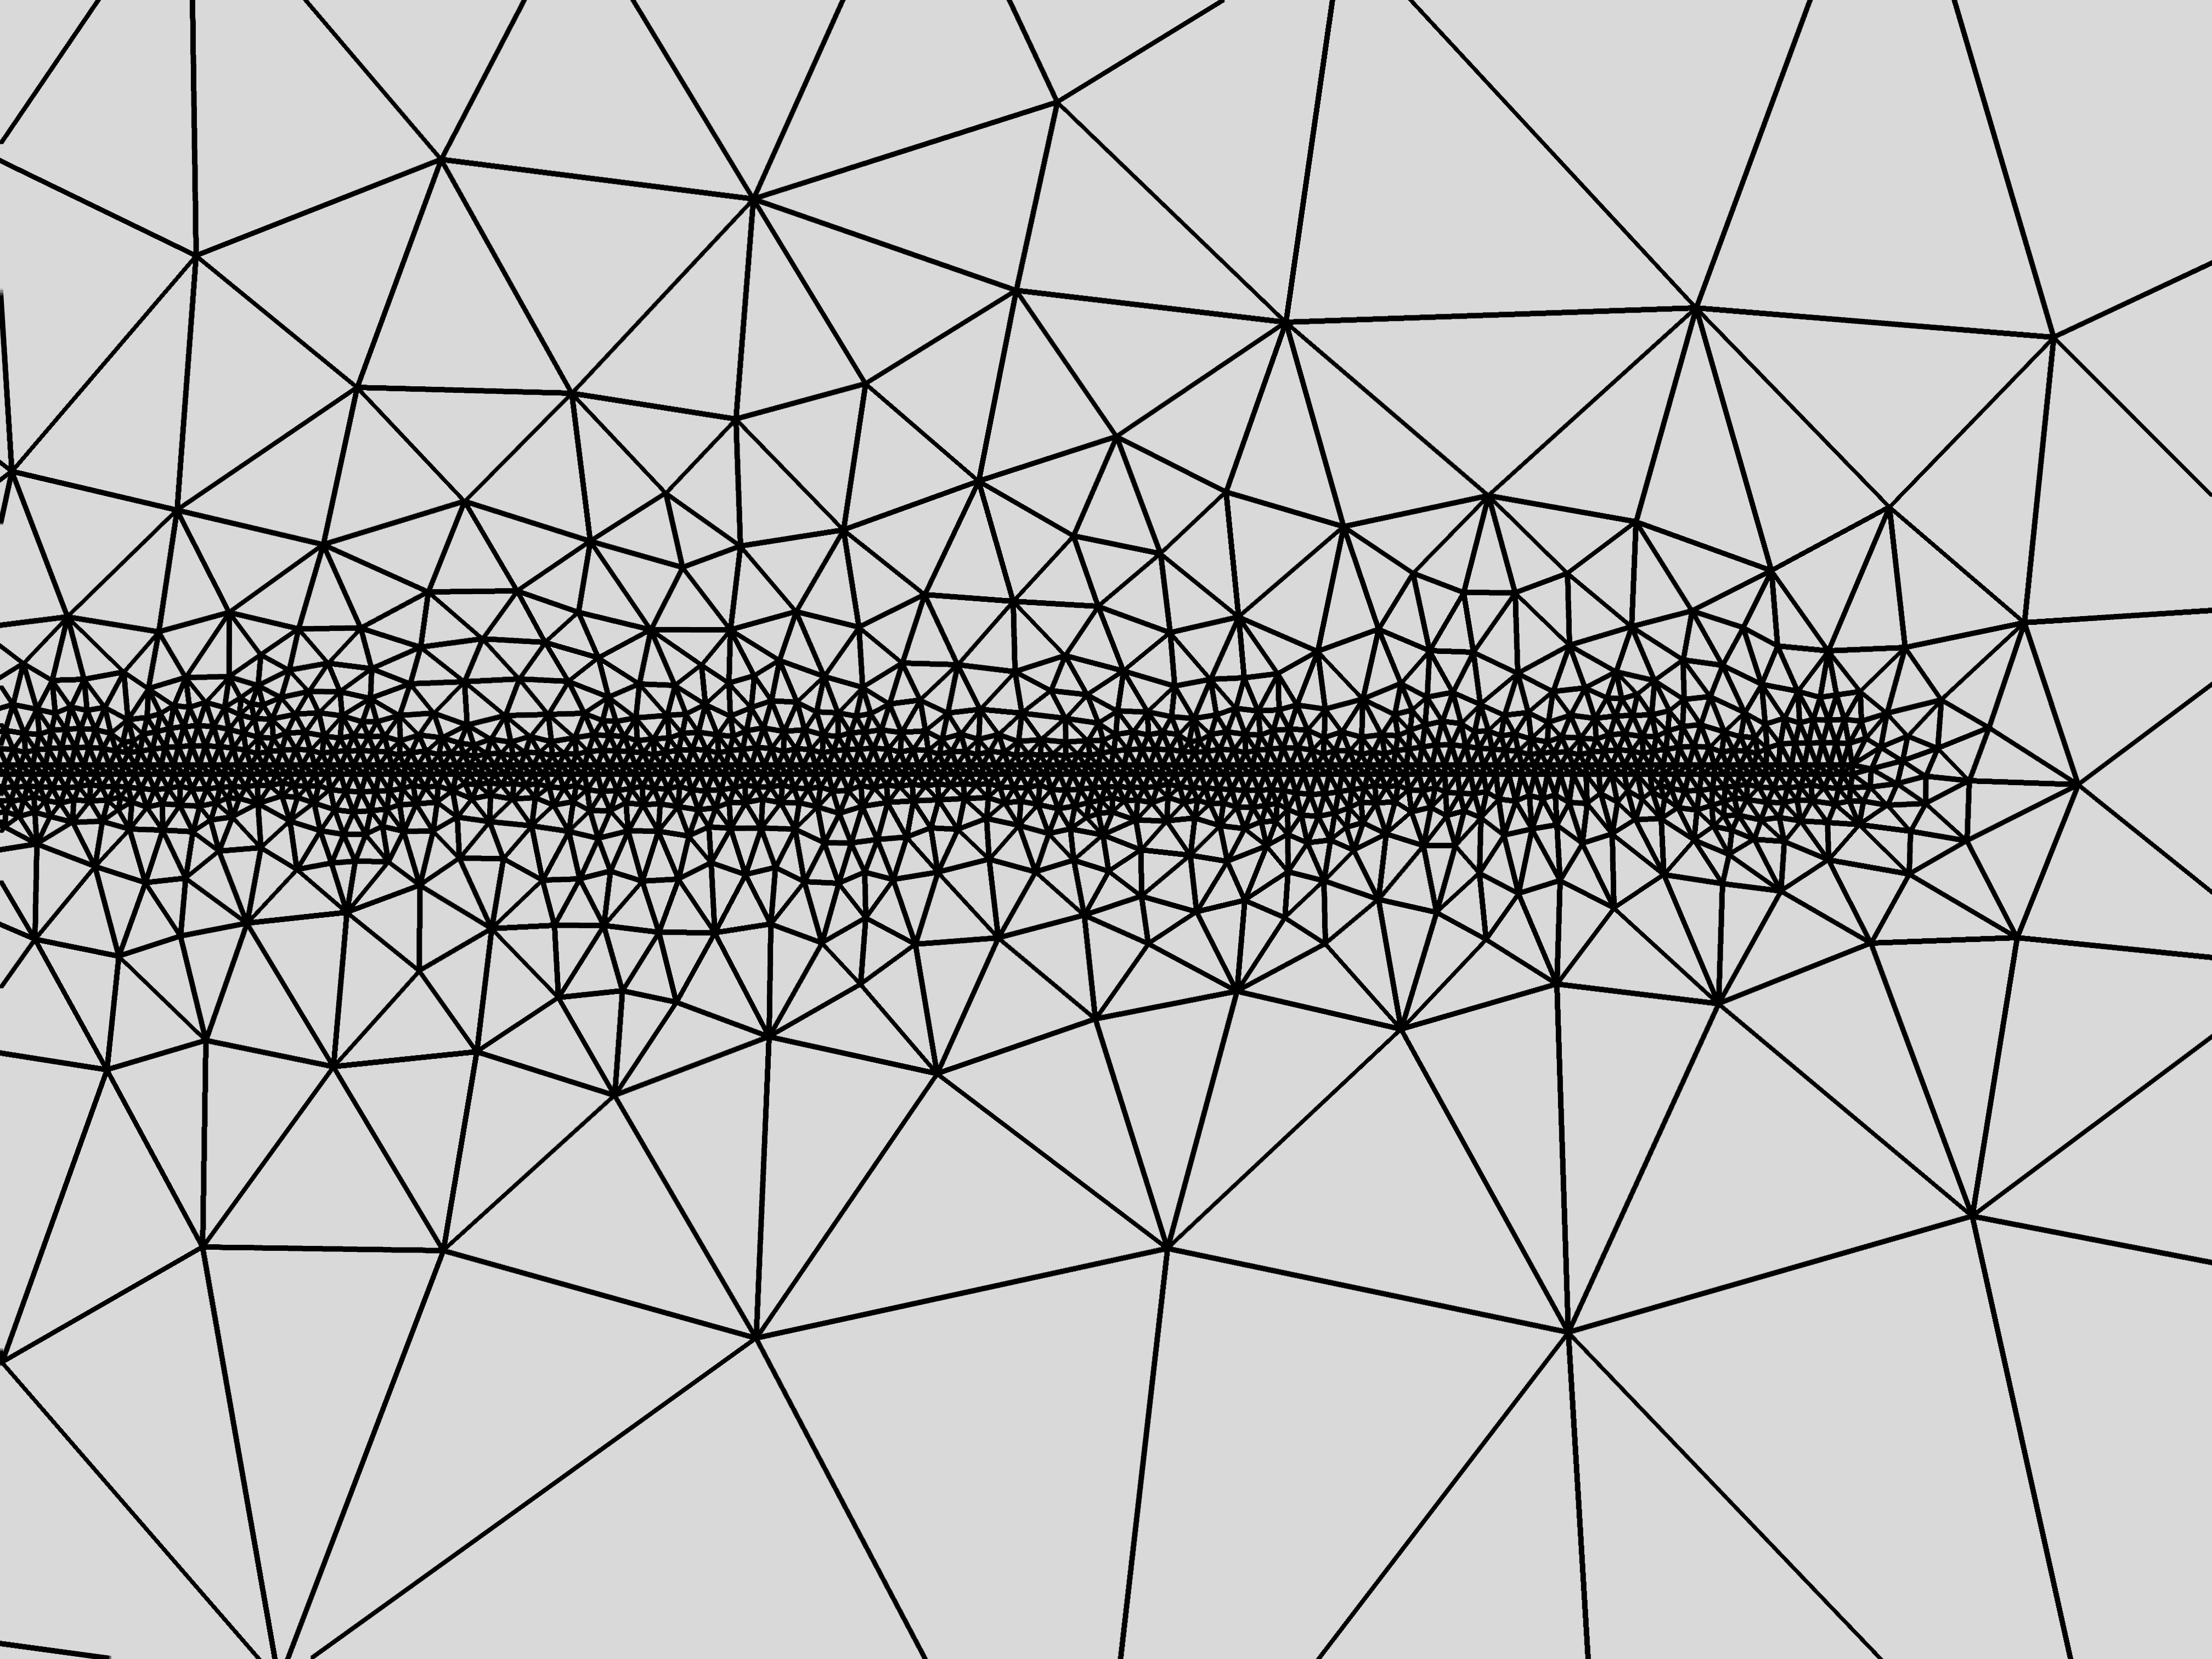
\includegraphics[width=1\textwidth]{figures/mesh.png}
           \caption{Typical mesh for a dielectric plate of thickness $.05 \u m$}
           \label{fig:mesh}
        \end{figure}
        \end{column}%
      \end{columns}
    \end{frame}
    % ------------------------------------------------------------
    % ------------------------------------------------------------
    % ------------------------------------------------------------
    % ------------------------------------------------------------
    % ------------------------------------------------------------
    % ------------------------------------------------------------
    % ------------------------------------------------------------
    \begin{frame}
      \frametitle{Field Computation}
      \framesubtitle{Integral Equations}
      \begin{columns} % align columns
        \begin{column}[T]{.5\textwidth}
          \begin{itemize}
            \item Difficulty in simulation of thin objects
            \item Dense mesh
            \item Computationally expensive
            \item No guarantee of correct solution
          \end{itemize}
        \end{column}
        \begin{column}[T]{.5\textwidth}
          \begin{figure}[!t]
             \noindent
             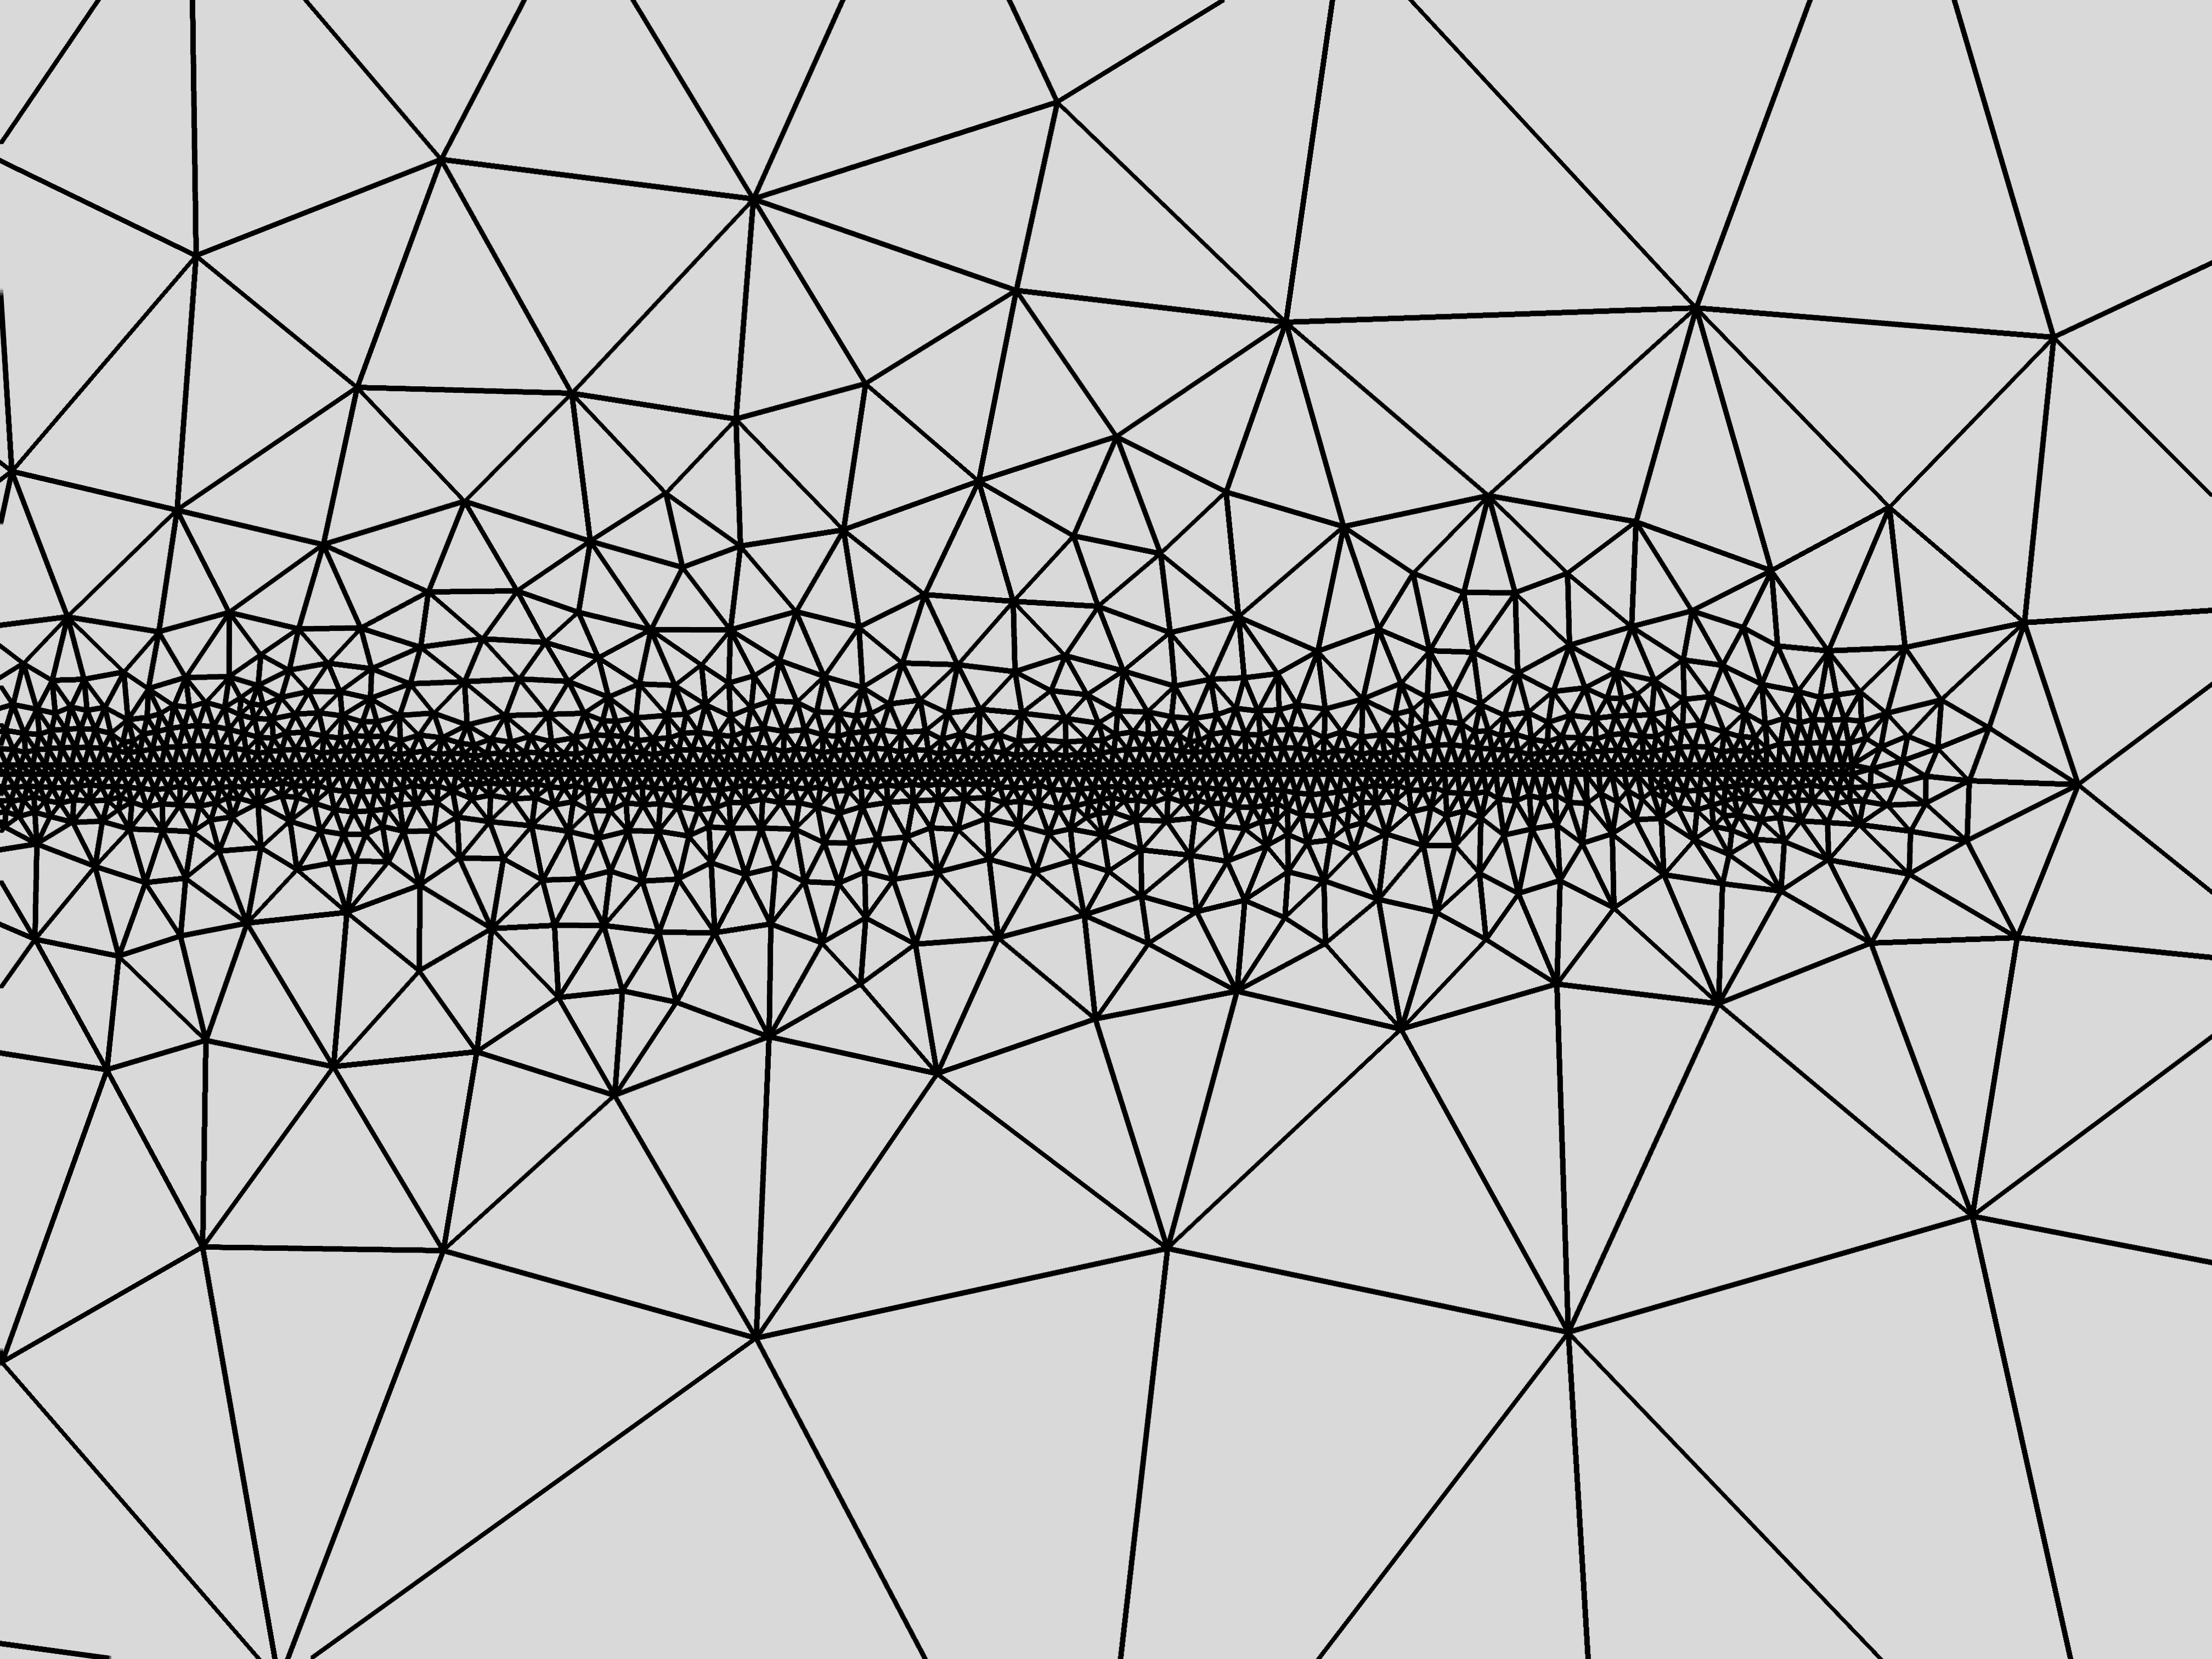
\includegraphics[width=1\textwidth]{figures/mesh.png}
             \caption{Typical mesh for a dielectric plate of thickness $.05 \u m$}
             \label{fig:mesh}
          \end{figure}
          \end{column}%
        \end{columns}
      \end{frame}
      % ------------------------------------------------------------
      % ------------------------------------------------------------
      % ------------------------------------------------------------
      % ------------------------------------------------------------
      % ------------------------------------------------------------
      % ------------------------------------------------------------
      % ------------------------------------------------------------
    \begin{frame}
      \frametitle{Proposed Scheme}
      \framesubtitle{Method of moments}
      \begin{itemize}
        \item {Integral equations to sytem of linear equations}
      \end{itemize}
      \[
      \begin{bmatrix}
        Z_{mn}   & 0 \\
        0        & Y_{mn}
      \end{bmatrix}
      \begin{bmatrix}
        J_n \\
        M_n
      \end{bmatrix}
      =
      \begin{bmatrix}
        E_m^i \\
        H_m^i
      \end{bmatrix}
      \]
      \begin{itemize}
        \item {Pulse basis functions and Point matching used}
        \item {Far-field}
      \end{itemize}
      \begin{equation} \nonumber
      RCS({\phi}) \simeq \int \limits_{0}^{L} \left[J_z(x')\eta_1 + M_x(x')\sin(\phi_i)\right] e^{j k_1 x' \cos(\phi_i)} \mathrm{d}x'
      \label{eq:far-field}
    \end{equation}
    \end{frame}
  % ------------------------------------------------------------
  % ------------------------------------------------------------
  % ------------------------------------------------------------
  % ------------------------------------------------------------
  % ------------------------------------------------------------
  % ------------------------------------------------------------
  % ------------------------------------------------------------
  \begin{frame}
    \frametitle{Two-dimensional Electon Gas (2DEG)}
    \framesubtitle{Existence of Surface Waves}
    \begin{columns} % align columns
      \begin{column}[T]{.5\textwidth}
        \begin{equation} \nonumber
          \E_1(\O) \cdot \E_2(\O) < 0
          \label{eq:conditions}
        \end{equation}
        \begin{itemize}
          \item Criterion met at terahertz frequency ra nge
          \item Opposite signs of dielectric constant at Semiconductor interface
          \item GaAs/AlGaAs semiconductor heterostructures
          \item Strontium Titanate/Lanthanum Aluminate (STO/LAO) oxide interfaces
        \end{itemize}
      \end{column}
      \begin{column}[T]{.5\textwidth}
        % \begin{figure}
        %   \vspace*{-2cm}
        %   \subfloat{\includestandalone[width=.75\linewidth,keepaspectratio]{figures/epsilon_gaas}
        %   \label{fig:eps_Ga}}
        %   \vspace*{0cm}
        %   \subfloat{\includestandalone[width=.75\linewidth,keepaspectratio]{figures/epsilon_sto}
        %   \label{fig:eps_Sto}}
        %   \caption{Dielectric Functions of the materials in bulk form. Solid line: real part, dashed line: imaginary part}
        %   \label{fig:eps}
        % \end{figure}
        \end{column}%
      \end{columns}
    \end{frame}

    \end{document}
